\begin{exercice*}
    Construire un triangle $A'B'C'$ isométrique au triangle $ABC$ en utilisant le côté $[A'B']$.

    Il y a deux solutions à tracer avec des couleurs distinctes.

        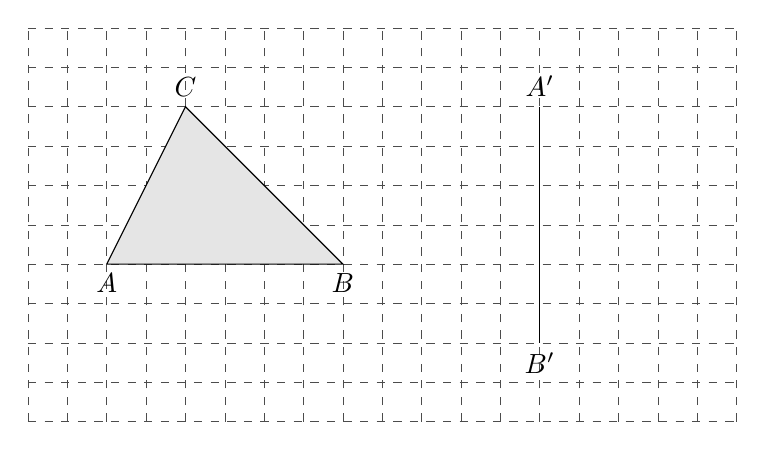
\begin{tikzpicture}[scale = 0.5]
            \draw[help lines, color=black!70, dashed] (0,0) grid (18,10);
            \coordinate[label=below:$A$] (A) at (2,4);
            \coordinate[label=below:$B$] (B) at (8,4);
            \coordinate[label=above:$C$] (C) at (4,8);
            \coordinate[label=above:$A'$] (A') at (13,8);
            \coordinate[label=below:$B'$] (B') at (13,2);            
            \draw[fill=gray!20] (A) -- (B) -- (C) -- (A);
            \draw (A') -- (B');
        \end{tikzpicture}
\end{exercice*}
\begin{corrige}
    %\setcounter{partie}{0} % Pour s'assurer que le compteur de \partie est à zéro dans les corrigés
    \phantom{rrr}    

    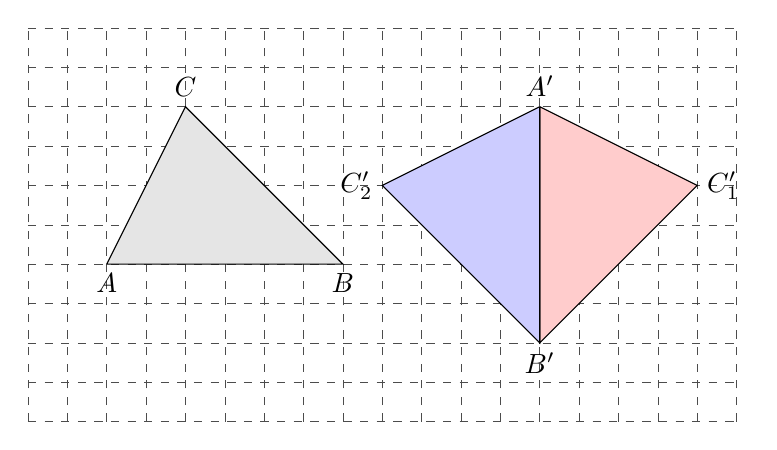
\begin{tikzpicture}[scale = 0.5]
        \draw[help lines, color=black!70, dashed] (0,0) grid (18,10);
        \coordinate[label=below:$A$] (A) at (2,4);
        \coordinate[label=below:$B$] (B) at (8,4);
        \coordinate[label=above:$C$] (C) at (4,8);
        \coordinate[label=above:$A'$] (A') at (13,8);
        \coordinate[label=below:$B'$] (B') at (13,2);
        \coordinate[label=right:$C_{1}'$] (C1) at (17,6);
        \coordinate[label=left:$C_{2}'$] (C2) at (9,6);        
        \draw[fill=gray!20] (A) -- (B) -- (C) -- (A);
        \draw[fill=red!20] (A') -- (B') -- (C1) -- (A');
        \draw[fill=blue!20] (A') -- (B') -- (C2) -- (A');

    \end{tikzpicture}
\end{corrige}

